\subsection{Brushless Motoransteuerung}

\begin{tabular}{p{3.6cm}p{9.4cm}}
\textit{Typ}              & Ballmaschine\\ 
\textit{Datum}:           & 22.11.2014\\
\textit{Ort}:             & Labor HSLU\\
\textit{Tester}:          & Yves Studer\\
\textit{Ziel des Testes}: & Testen ob die Ansteuerung eines Brushless Motors in verhältnismässiger Zeit realisierbar ist. Weiter wird versucht, die Signale von Hallsensoren aus der Ansteuerung zu rekonstruieren, da die Steuerung des Motors mittels Hall-Sensoren einfacher realisiert werden kann.\\
\textit{Fazit / Verbesserungs-\newline vorschlag}: & Die Ansteuerung des Motors ist mit erstaunlich wenig Aufwand möglich. Den Motor drehen lassen ist kein Problem. Ob das maximale Drehmoment erreicht werden kann, bedarf weiteren Abklärungen. Im Versuchsaufbau konnte mit einer Wirbelstrombremse rund 100W elektrischer Leistung im Motor umgesetzt werden. \\ 
\textit{Ziel erreicht}:& Ja\\
\end{tabular}\\
\\
\\
\textbf{Aufbaubeschreibung}:
\begin{wrapfigure}{r}{0.55\textwidth}
	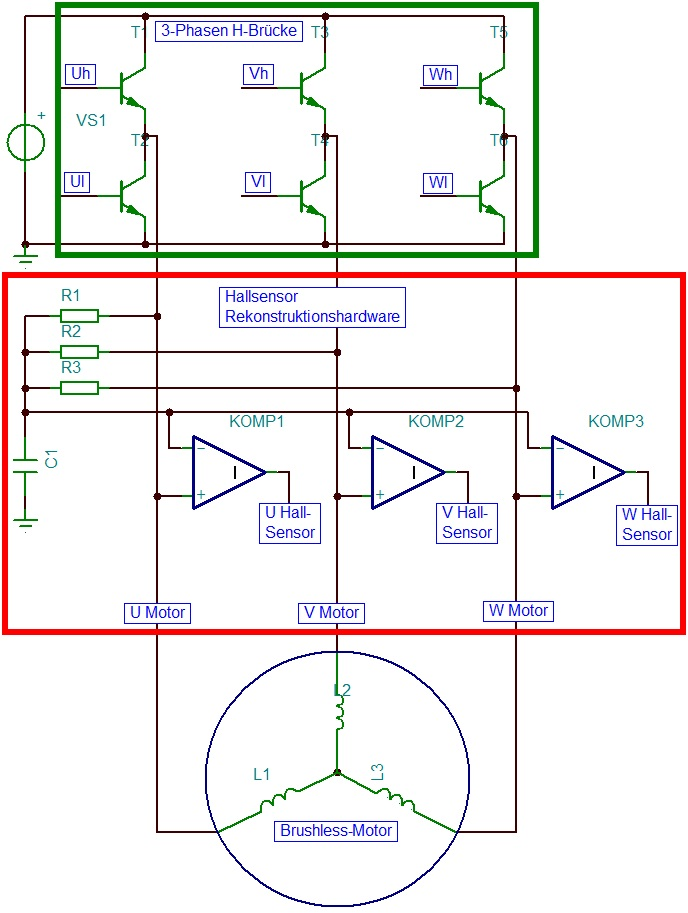
\includegraphics[scale=0.4]{Funktionstests/Bilder/MotoransteuerungSchema.jpg}
	\centering
	\caption{Schema des Brushless-Versuchsaufbaus}
\label{abb:MotoransteuerungSchema}
\end{wrapfigure}
Das Schema des gesamten Aufbaus des Tests ist in der Abbildung \ref{abb:MotoransteuerungSchema} abgebildet. Die 3-Phasen H-Brücke oben im grünen Rechteck wird direkt vom FPGA angesteuert. Die Hardware dieser Brücke ermöglicht eine voll galvanisch getrennte Ansteuerung mit 3.3V Logikpegeln. Diese Brücke wurde zur Verfügung gestellt und verwendet. Die Rekonstruktion der Hallsensoren-Signale findet im rot markierten Teil des Aufbaus statt. Dieser Part wurde auf einer Laborplatte aufgebaut und zusammen gelötet. Die so generierten Signale $U_{Hallsensor}$, $V_{Hallsensor}$, $W_{Hallsensor}$ werden einem FPGA geliefert. Anhand dieser Signale steuert dieses das FPGA die H-Brücken-Transistoren mittels der Signale $U_h$, $U_l$, $V_h$, $V_l$, $W_h$, $W_l$. Die im FPGA enthaltene Konfiguration sind simple AND-Verknüpfungen, die die anligenden Signale sehr schnell und effizient verarbeiten. Auf diese Weise ist es möglich, den Motor sehr schnell anzusteuern.\\
\\
In der Abbildung \ref{abb:MessplatzAufbau} ist der gesamte Aufbau abgebildet. Man beachte die markierten Felder. am unteren linken Rand ist der Motor befestigt. In der Mitte des Bildes ist die Hardware, mit der die Hallsensoren Signale rekonstruiert werden. Die generierten Signale werden dem FPGA in der unteren linken Ecke zugeführt. Diese Signale werden logisch verknüpft und danach werden die sechs Signale generiert um die H-Brücke in der oberen rechten Hälfte anzusteuern. Diese Wiederum treiben den Motor an.\\
\begin{figure}[h!]
%\vspace{-16pt}
	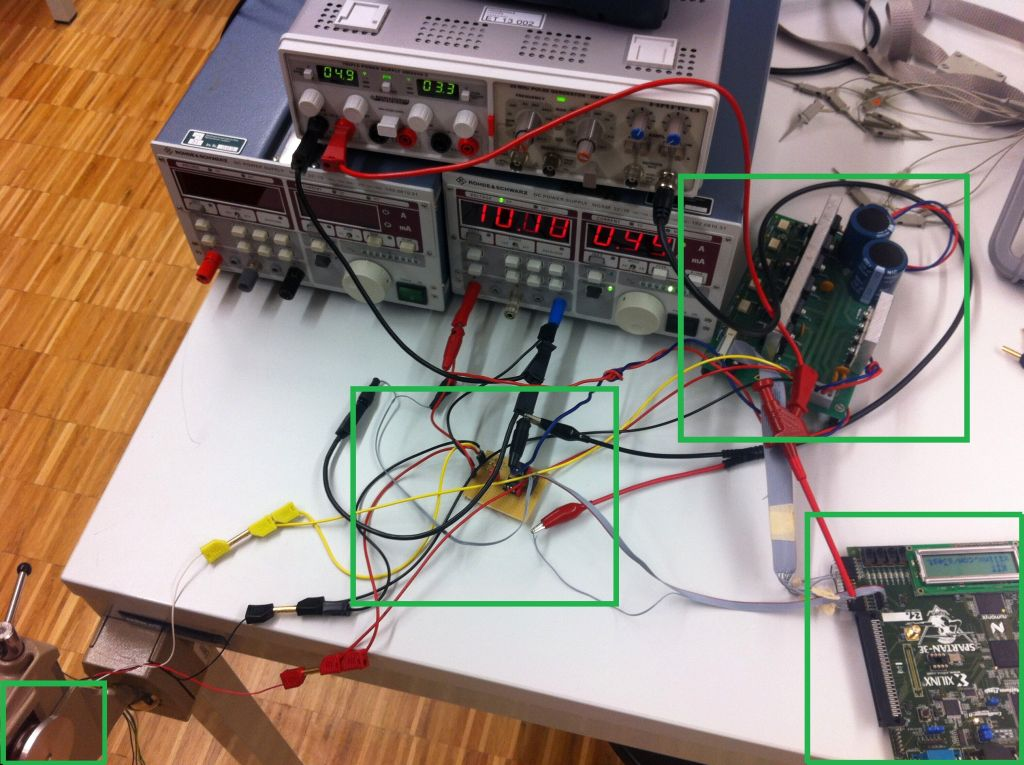
\includegraphics[scale=0.14]{Funktionstests/Bilder/MessplatzAufbau.jpg}
	\centering
	\caption{Schema des gebauten Boards} 
\label{abb:MessplatzAufbau}
%\vspace{-10pt}
\end{figure}